\chapter{物质的状态与状态变化}\label{ch:g7:states-of-matter}

六年来，固体保持形状，液体保持水平，
气体充满每个角落——而我们从未追问
\emph{为什么}。这一年，物理学掀开了盖子。三态之下
隐藏着人类最伟大的思想之一：万物，
无一例外，都由小到肉眼无法看见的粒子组成。只要接受这一思想，
你自幼积累的那些规律
便都能一气呵成地得到解释。

\section{伟大的思想}

\begin{definition}[分子]\label{def:g7:states-of-matter:molecule}
一切物质都由\emph{分子}\index{分子}构成：
分子极其微小，远小于肉眼或学校显微镜
所能看到的尺度。一滴水中的分子数，
比全世界海洋中的水滴数还多。每种纯净物质
都由其特有的分子构成——水由水分子构成，
铁由铁的分子构成——同一种物质的分子
完全相同。
\end{definition}

\begin{remark}[不见而信]\label{rem:g7:states-of-matter:believing}
没有人曾用肉眼看到过一个分子——
那么为何要相信它们呢？因为这一思想\emph{值得}信赖：它
能正确预言本章的全部内容，以及
更多的内容。物理学正是这样接纳一位看不见的“客人”：
不靠信仰，而靠持续不断的实用价值。（直接拍到分子图像的
精妙现代仪器，直到一个世纪前才出现——
那时物理学家早已确信。）
\end{remark}

\begin{proposition}[三态的粒子模型]\label{prop:g7:states-of-matter:model}
三种状态是同一种分子的三种排列方式：
\begin{enumerate}
  \item \emph{固体}：分子紧密有序地排列成
        一堆，每个分子在原处振动，但位置固定，
        因此形状固定；
  \item \emph{液体}：分子仍然相互接触，但排列无序，
        可以彼此滑过——因此能够流动，
        并形成水平的液面；
  \item \emph{气体}：分子相距很远，向各个方向快速运动，
        相互碰撞并弹开——因此
        能充满所提供的每个角落。
\end{enumerate}
\end{proposition}

\begin{omfigure}
\begin{tikzpicture}[scale=0.8]
  \draw[thick] (0,0) rectangle (3.2,3.0);
  \foreach \i in {0,...,6} {
    \foreach \j in {0,...,5} {
      \fill[omDef] (0.34+\i*0.42,0.32+\j*0.45) circle (0.13);
    }
  }
  \node[below, font=\small] at (1.6,-0.3) {固体：有序，位置固定};
  \draw[thick] (4.4,0) rectangle (7.6,3.0);
  \foreach \x/\y in {0.4/0.3, 0.85/0.62, 1.3/0.28, 1.75/0.55,
      2.2/0.3, 2.65/0.6, 2.9/0.32, 0.5/1.0, 1.0/1.15, 1.5/0.95,
      2.0/1.1, 2.5/1.02, 2.85/1.25, 0.42/1.55, 0.95/1.7,
      1.45/1.5, 1.95/1.65, 2.45/1.55, 0.6/2.1, 1.2/2.2, 1.8/2.05,
      2.4/2.15} {
    \fill[omDef] (4.4+\x,\y) circle (0.13);
  }
  \node[below, font=\small] at (6.0,-0.3)
    {液体：相互接触，可滑动};
  \draw[thick] (8.8,0) rectangle (12.0,3.0);
  \foreach \x/\y/\a in {0.5/0.5/40, 1.6/1.1/160, 2.7/0.4/95,
      0.7/1.9/-30, 1.9/2.4/210, 2.9/1.7/120, 1.2/2.8/-70} {
    \fill[omDef] (8.8+\x,\y) circle (0.13);
    \draw[-Stealth, omExo] (8.8+\x,\y) -- ++(\a:0.55);
  }
  \node[below, font=\small] at (10.4,-0.3)
    {气体：相距很远，飞速运动};
\end{tikzpicture}

{\small 同一种物质，三种排列：堆叠的固体，
液体中可滑动的分子群，气体中飞动的稀疏分子。}
\end{omfigure}

\begin{example}[六年规律，一种解释]\label{ex:g7:states-of-matter:rules}
用这一模型检验旧有的规律。固体保持形状：
每个分子各守其位。液体取容器的形状，
并保持水平：可滑动的分子群下沉，直到没有分子能
再向下滑动。气体充满所提供的全部空间：没有任何东西
拦住飞动的分子。香水在房间里扩散：气体分子飞动、
碰撞、扩散。沙子像液体一样倾泻：流动的不是分子，
而是沙粒——每一粒沙本身就是一个由
万亿个分子组成的微小有序固体。
\end{example}

\section{空隙检验}

\begin{method}[两个注射器]\label{met:g7:states-of-matter:syringe}
该模型认为：气体分子飞得很远，液体分子
相互接触。于是气体应可被压缩，液体则不应。对此加以检验：
\begin{enumerate}
  \item 将塑料注射器充满空气，用指尖堵住针口，
        推动活塞：活塞会移动——你可以
        将空气的体积压缩一半，并感受到有弹性的反推力；
  \item 将同一注射器充满水，堵住针口后推动：活塞
        像一堵墙一样纹丝不动——水连细微的一点
        都不肯被压缩；
  \item 松开每个活塞：空气的活塞弹回；水的
        活塞从未移动。
\end{enumerate}
\end{method}

\begin{proposition}[气体可被压缩；液体和固体不能]\label{prop:g7:states-of-matter:squeeze}
气体可以被\emph{压缩}\index{压缩}——被压入
更小的空间中——因为气体的大部分是飞动分子之间的
空隙。液体和固体实际上
是\emph{不可压缩}的：它们的分子已经相互接触，
而相互接触的物质，无论用多大的推力——
哪怕是一只手或一台液压机——都无法将其压得更紧。
\end{proposition}

\begin{example}[被压缩的空气大显身手]\label{ex:g7:states-of-matter:squeezed}
自行车打气筒把满满一屋子的空气压进轮胎——
只因为空气大部分是空隙，这才办得到。被压缩的
分子群更快、更密集地撞击轮胎内壁，
撑起了自行车：气体的推力\emph{就是}它的分子冰雹。
潜水员的气瓶把一下午的呼吸量压进一只
钢瓶里；而不可压缩的刹车油则把脚下的推力
原样传到车轮上——
各种状态各尽其长。
\end{example}

\section{状态变化重温}

\begin{example}[六扇门，从分子看]\label{ex:g7:states-of-matter:doors}
加热固体，其颤动的分子振动得更加剧烈；在熔点处，
剧烈的振动冲破了有序的堆叠——人群开始滑动：熔化。
继续加热液体，速度最快的分子
会彻底挣脱人群的束缚而飞出：
蒸发——到达沸点时，逃逸之势化为
从液体内部涌出的一场“逃逸狂潮”。冷却让这部影片倒放：
飞走的分子被捕获（液化），
滑动的分子锁入队列（凝固）。去年学过的六扇门，
其实是同一个故事：分子束缚与分子振动的较量。
\end{example}

\begin{example}[两条旧定律，不费力便得]\label{ex:g7:states-of-matter:free}
两条来之不易的定律如今不费吹灰之力即可得到。\emph{质量在状态变化中
保持不变}：熔化只是重排分子，既不产生也不消灭任何一个分子——
粒子相同，质量也相同。
\emph{温度保持不变}：在熔点处，流入的热量用于
拆散堆叠的束缚，一个分子接一个分子，而不是用于加快振动——
温度计要等到最后一排被拆散后才会变化。
测量所发现的，模型都能解释。
\end{example}

\begin{remark}[水的反常膨胀]\label{rem:g7:states-of-matter:iceswell}
甚至水的奇特结冰膨胀也来凑热闹：水分子
恰好会锁成一种异常\emph{疏松}的堆叠——
一种开放的晶格，空隙比滑动的分子群更多。
堆叠越疏松、空间越大、密度越低：冰漂浮在它自身的液体上。
大多数物质的堆叠比其滑动时更紧密；
水的结构则是一个美妙的例外。
\end{remark}

\begin{omfigure}
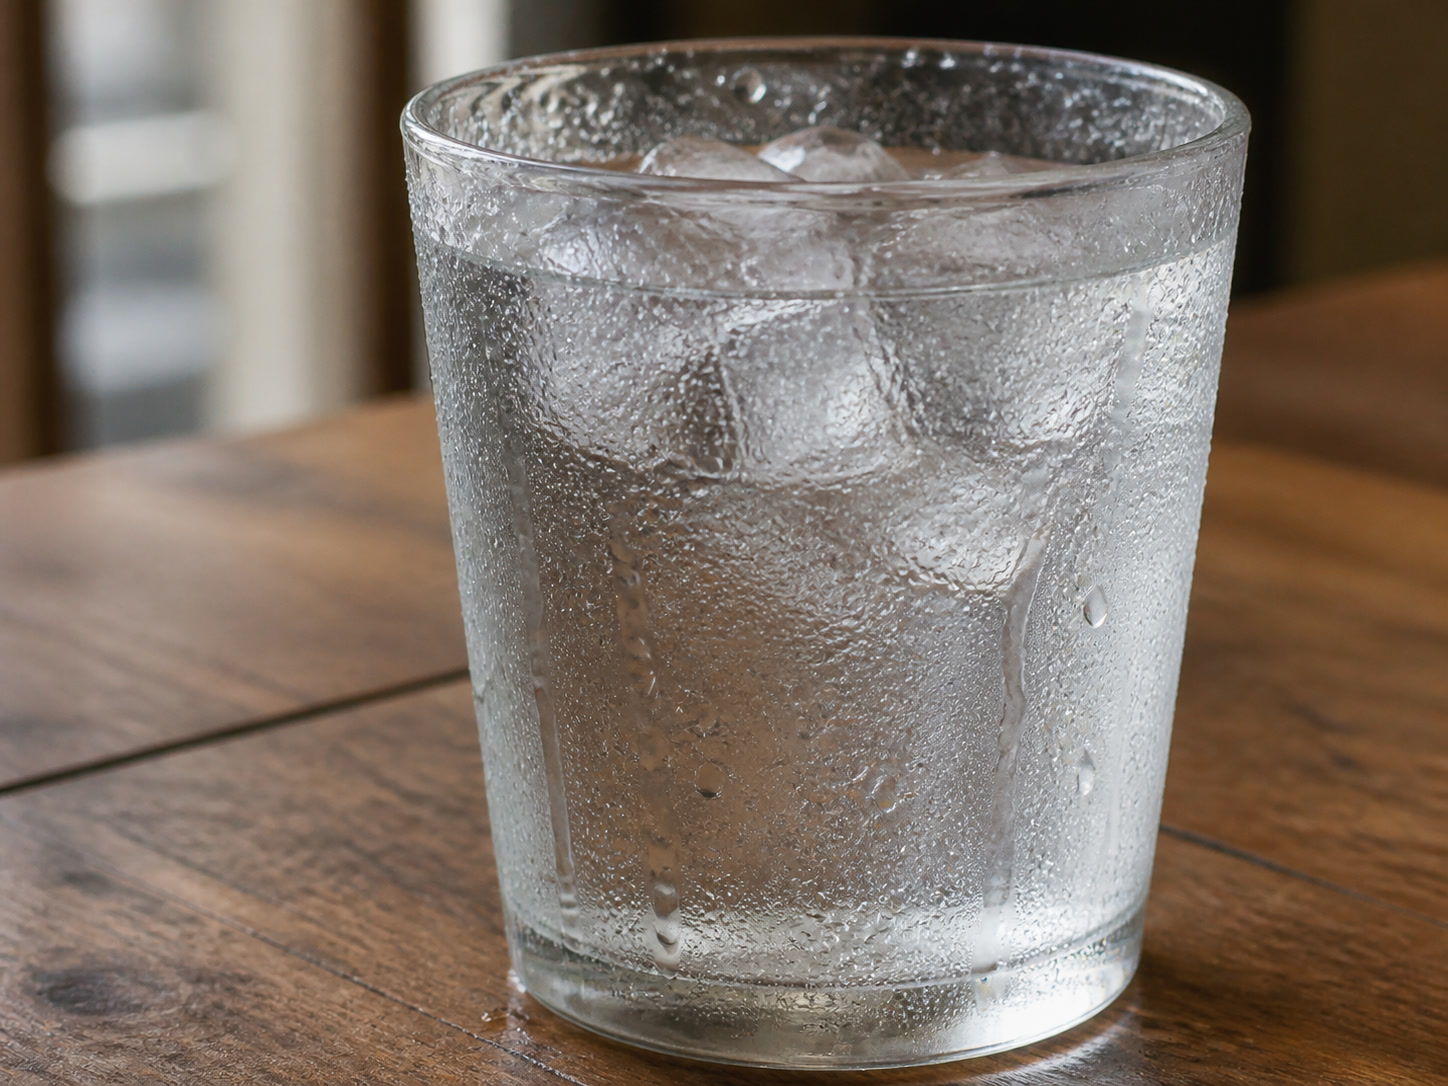
\includegraphics[width=0.5\linewidth]{images/book1/ai/g7-states-dew.jpg}

{\small 正在发生的液化：房间空气中看不见的水蒸气在冷玻璃上变成液体。}
\end{omfigure}

\section{从内部看热量}

\begin{proposition}[温度与分子运动]\label{prop:g7:states-of-matter:temperature}
温度衡量分子运动的活跃程度：物质越热，
其分子颤动、滑动或飞动得越快。热量从高温流向低温，
是活跃的分子群在一次次碰撞中安抚迟钝的分子群，
直到二者步调一致，达到同一温度。
热量“顺坡而下”的旧规律，
不过是分子间的乒乓球游戏。
\end{proposition}

\begin{example}[冷不是一种物质]\label{ex:g7:states-of-matter:cold}
模型永久地抛弃了一种旧观念：
从来没有一种叫“冷”的东西在流动。
只有分子运动的快慢之分；活跃的分子只会把活跃传出去，
绝不会反过来。在可以想象的最冷状态——分子尽可能静止，
那里有温度真正的下限，远低于任何冷库；
其奇特而著名的数值属于高中分册。
\end{example}

\section{练习}

\begin{exercise}[$\star$]\label{exo:g7:states-of-matter:1}
用粒子模型描述三种状态各自的图景，
每种状态各用一行作答。
\end{exercise}

\begin{exercise}[$\star$]\label{exo:g7:states-of-matter:2}
为什么固体能保持形状，而液体却取容器的形状？
请用分子来解释，而不要用规则。
\end{exercise}

\begin{exercise}[$\star$]\label{exo:g7:states-of-matter:3}
在注射器实验中，为什么空气会被压缩、随后回弹，
而水却像一堵墙一样纹丝不动？
\end{exercise}

\begin{exercise}[$\star$]\label{exo:g7:states-of-matter:4}
自行车打气筒能把许多屋子的空气压进一个轮胎。
这说明了气体分子间距的什么特性？
能否用打气筒对水做同样的事？
\end{exercise}

\begin{exercise}[$\star$]\label{exo:g7:states-of-matter:5}
用分子语言讲述熔化的过程：热量做了什么，
在熔点处又是什么被打破？
\end{exercise}

\begin{exercise}[$\star$]\label{exo:g7:states-of-matter:6}
根据该模型，为什么
每次状态变化中质量都保持不变？若要使质量
减少，分子需要发生怎样的变化？
\end{exercise}

\begin{exercise}[$\star$]\label{exo:g7:states-of-matter:7}
在该模型中，温度衡量的是什么？描述热量
顺坡流动的过程，并将其比作分子乒乓球游戏。
\end{exercise}

\begin{exercise}[$\star$]\label{exo:g7:states-of-matter:8}
在一间静止空气的房间一端打开香水，
一分钟后另一端就能闻到。请解释这一过程，
并说明为什么微风会使其加快。
\end{exercise}

\begin{exercise}[$\star\star$]\label{exo:g7:states-of-matter:9}
蒸发使留下的液体降温：汗水使皮肤变凉，
把湿手指伸向风中，能感到风较凉的一面。请用
\emph{最快的}分子逸出来解释——
留下的是怎样的一群分子？
\end{exercise}

\begin{exercise}[$\star\star$]\label{exo:g7:states-of-matter:10}
一只密封的气球放在夏日阳光下会膨胀；放在
冰箱里则会变瘪。其内部分子的数目从未
改变。请用分子的速率以及
器壁上如冰雹般的撞击，解释这两种变化。
\end{exercise}

\begin{exercise}[$\star\star$]\label{exo:g7:states-of-matter:11}
用分子语言说明：冰为什么会漂浮？水分子
所形成的堆积方式有何异常？若水像普通物质那样堆积，
池塘在冬季会怎样？
\end{exercise}

\begin{exercise}[$\star\star\star$]\label{exo:g7:states-of-matter:12}
将一滴墨水轻轻放在盛有
\emph{静止的}水的杯底，经数小时缓慢扩散，直到
整杯水都微微发蓝——没有搅拌，也没有对流。请解释
这种缓慢的扩散揭示了液体分子的哪些性质，
既包括水的分子，也包括墨水的分子，以及为什么同样一滴墨水
在温水中扩散得更快。（这一朴素的观察，曾是
分子学说早期最重要的证据之一。）
\end{exercise}

\section{问题：分子剧场}

\begin{problem}[{周末问题——全班在体育馆演绎粒子
模型：学生扮演分子，物态作为动作设计；评论者的
问题}]\label{pb:g7:states-of-matter:1}
物理课全班要演出物质本身：三十名学生扮演
同一种物质的分子，体育馆就是容器。

\medskip\noindent\textbf{三幕场景。}
\begin{enumerate}
  \item 第一幕，固体：三十名学生应当如何站立，以及
        每个人必须持续做怎样的微小运动？有什么
        是任何人都不能做的？
  \item 第二幕，液体：排列方式发生了什么变化，
        出现了什么新的活动自由？学生们仍须保持哪些
        将在气体一幕中被取消的动作？
  \item 第三幕，气体：描述其编排——并
        说明为什么这一幕需要\emph{整个}体育馆，而前两幕
        只需挤在一角。
  \item 观众提问：“三幕中的学生是否
        始终是同一批三十名学生？”这个答案
        体现的是去年学过的哪条定律？
\end{enumerate}

\medskip\noindent\textbf{第二部分——评论者检验这出戏。}
\begin{enumerate}[resume]
  \item 一位评论者轻轻推动气体一幕中的人群，
        将其挤进半个体育馆。这一幕允许这样吗？同样的
        推力作用于液体一幕中挤作一团的人群时呢？请说出
        所要演示的命题。
  \item 要演出\emph{熔化}，导演设定了一个
        假想的热量旋钮。固体一幕中的学生必须
        越来越多地做什么？在哪个时刻，这一幕
        才算成为液体一幕？
  \item 这出戏必须展示熔化平台：变化进行时，
        热量旋钮提供的能量用于什么——并
        “温度计评论员”必须报告这段时间内学生的
        平均运动剧烈程度有何变化？
  \item 在液体一幕中演出蒸发：哪些学生
        离开人群——是随机的任何人，还是特定的
        某一类？随着他们离开，人群的平均活跃程度
        会怎样变化？这解释了哪种日常的凉意？
\end{enumerate}

\medskip\noindent\textbf{第三部分——特殊效果。}
\begin{enumerate}[resume]
  \item 气球效果：气体一幕由手持绳环的学生围住
        （绳环代表气球的表皮）。分子演员对绳子
        做了什么？当演员运动得更快时，绳环会
        发生什么变化？
  \item 水的反常凝固必须演出：导演对固体一幕的
        堆叠给出了关于\emph{间距}的哪条不寻常指令？
        这条指令还解释了哪一个漂浮事实，
        并予以说明？
  \item 墨水滴的终场：一名穿蓝衬衫的学生从
        \emph{液体}一幕的角落出发。没有任何
        导演的推动，这名蓝衬衫学生如何远离
        出发的角落——热量旋钮调高时为何会更快？
  \item 撰写节目说明：用三句话说明整出戏演示的是哪一个
        核心思想，指出它能顺便解释的两条旧定律，
        并坦率承认任何一幕都无法呈现的内容
        （真实的分子演员
        有多\emph{小}、有多\emph{多}）。
\end{enumerate}
\end{problem}
